\chapter{Model}

%In this chapter we formulate two models of substance abuse that are very similar and only differ with regard to the component that describes the force of infection. The first model assumes that the factor influencing initiation after contact between a susceptible and a substance abuser is innovation on the part of the susceptible. \citep{Bruno} describe the innovators as that type of individuals who make a decision to adopt a certain other people in the society or their interaction with peers.
%
%The other model assumes that the factor at play in the individuals that are recruited from the susceptible population to the drug users population is imitation. \citep{Bruno} also gives a description of these individuals as adopters who respond  to the pressure of their environment and thus it influences the timing of innovation not necessarily depending on the decision of their adoption.

In formulating the age structured model of substance abuse  we introduce the following parameters :

\begin{table}[h!]
\centering
\begin{tabular}{|c|l|}\hline
\text{Parameter} &\text{ Description}\\ \hline 
N(a,t) & \text{Expected population size  of age $a$ at time $t$}\\
\beta(a,t) & \text{The effective contact rate of age $a$ at time $t$}.\\
\mu (a) & \text{The per capita death rate as a function of age} \\
\sigma (a) & \text{The rate of movement into rehabilitation} \\
\gamma (a) & \text{The rate of relapsing while in rehab}\\
\rho(a) & \text{The recovery rate}\\
\omega (a) & \text{The relapse rate of the recovereds}\\
\alpha (a) & \text{The imitation coefficient} \\
\hline 

\end{tabular}
 \caption{The table gives the model parameters and their description.}
\end{table}







%N is a large positive integer, $\beta$ and $\mu$ are positive.
%\text{Parameter} &\text{ Description}\\ 
%N & \text{Expected population size  in case there are no infected individuals}\\
%
%
%\beta &\text{The contact rate between infectives and susceptibles}.\\
%\mu & \text{The death rate and the birth rate} \\
%\sigma & \text{The rate of movement into rehabilitation} \\
%\gamma & \text{The rate of relapsing while in rehab}\\
%\rho & \text{The recovery rate}\\
%\omega & \text{The relapse rate of the recovereds}\\
%\alpha & \text{The imitation coefficient} \\
%\end{array} \]


\section{Model Formulation}
Here we formulate a model that monitors four populations in relation to substance abuse. The first group consist of individuals  susceptible to substance abuse denoted by $S(a,t)$. These are individuals that are recruited into the population through birth. The second group is a group of drug users that are not in rehabilitation and that is denoted by $D(a,t)$. These individuals are initiated into drug use from the susceptible group. The  third compartment consists of individuals who are in rehabilitation having been in compartment $D(a,t)$ . The last compartment $Q(a,t)$ consists of individuals who have stopped using drugs and they are called  quitters. The total population is thus given by \[N=N(a,t)=S(a,t)+D(a,t)+R(a,t)+Q(a,t).\]
%Since the birth rate is equal to the death rate,  the population is assumed to be constant thus we have \[\frac{dN(t)}{dt}=0.\]
%This implies that \[\frac{dS(t)}{dt}+\frac{dD(t)}{dt}+\frac{dR(t)}{dt}+\frac{dQ(t)}{dt}=0.\]

The main assumption of this model is that the population is approximately constant within the modelling time. We also assume that that there is a homogeneous mixing among all individuals from different compartments. The class responsible for initiation is $D(a,t)$ which consists of drug users not in treatment. Drug users who are undergoing treatment in compartment $R(a,t)$ are assumed not to initiate new cases  since we assume that the rehabilitation is inpatient. We also assume that the susceptible class $S(a,t)$ consists of people who have never been involved in abusing substances before. Thus those who quit do not necessary move back to $S(a,t)$ but there is a possibility that they can still relapse and move straight back into $D(a,t)$. We now give the description of the dynamics of all compartments. The description is aided by  figure \ref{diagram}.

\begin{figure}[h!]
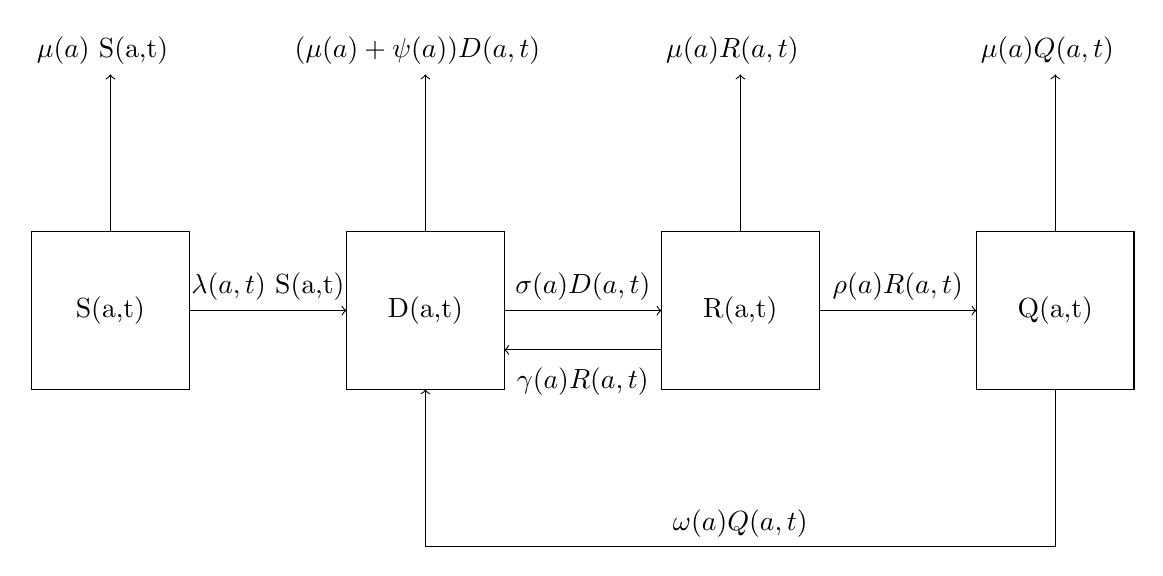
\begin{tikzpicture}
%\draw [->](-2,1) -- (0,1);
\draw  (0,0)rectangle(2,2) ;
\node (S) at (1,1) {S(a,t)};
\draw  (4,0)rectangle(6,2);
\node (D) at (5,1) {D(a,t)};
\draw  (8,0)rectangle(10,2);
\node (R) at (9,1) {R(a,t)};
\draw  (12,0)rectangle(14,2);
\node (Q) at (13,1) {Q(a,t)};
\draw [->] (2,1) -- (4,1);
%\node (1) at (-3,1) {$\mu$ N};
\draw [->] (6,1) -- (8,1);
\draw [->] (10,1) -- (12,1);
\draw [-] (13,0) -- (13,-2);
\draw [-] (13,-2) -- (5,-2);
\draw [->] (5,-2)--(5,0);
\draw[->](1,2) -- (1,4);
\node (2) at (0.9,4.3) {$\mu(a)$ S(a,t)};
\node (3) at (3,1.3) {$\lambda(a,t)$ S(a,t)};
\draw[->] (5,2) -- (5,4);
\draw[->] (9,2) -- (9,4);
\draw[->] (13,2) -- (13,4);
\draw[->] (8,.5) -- (6,.5);
\node (4) at (7,1.3) {$\sigma(a) D(a,t)$};
\node (10) at (7,.1) {$\gamma(a) R(a,t)$};
\node (5) at (11,1.3) {$\rho(a) R(a,t)$};
\node (6) at (4.9,4.3) {$(\mu(a)+\psi(a))D(a,t)$};
\node (7) at (8.9,4.3) {$\mu(a) R(a,t)$};
\node (8) at (12.9,4.3) {$\mu(a) Q(a,t)$};
\node (9) at (9,-1.7) { $\omega(a) Q(a,t)$};
\end{tikzpicture}
\caption{The diagrammatic representation of the substance abuse model with the compartments densities S(a,t),D(a,t),R(a,t),Q(a,t) and $\mu(a), \gamma(a), \sigma(a), \omega(a), \lambda(a), \rho(a)$ denoting the transition rates which are $\geq 0.$\label{diagram}}  
\end{figure}

\subsection{Susceptible Individuals, S(a,t)}
This is a group of individuals who are at risk of getting addicted to drugs. Individuals in this compartment have no history of substance abuse. Recruitment  into the susceptible compartment is due to births that are denoted by the boundary condition given below. Susceptible individuals initiated into substance abuse with an initiation function $\lambda(a,t)$ that is synonymous to the force of infection in disease models . The susceptible population is depleted through natural death plus disease induced death.
% Our general equation for this compartment is thus given as:
%\begin{eqnarray}\label{eq:sus}
%\frac{dS}{dt} & = &\mu N -\mu S - \lambda S 
%\end{eqnarray}

%%We are going to consider two forces of initiation. For the first one we assume that the force that drives the susceptibles into the drug using state is innovation on the the part of the susceptible individual due to interaction with individuals in $D$. The force of initiation is given as $\frac{\beta D}{N}$. 
The differential equation explaining the dynamics of the susceptible population is
 \begin{eqnarray}\label{inovation}
 \frac{\partial S(a,t)}{ \partial t}+ \frac{\partial S(a,t)}{\partial a} & = & -\mu(a) S(a,t) -\lambda(a,t)S(a,t). 
 \end{eqnarray}


%We also consider the case where the susceptible population is assumed to be recruited mainly through imitation.We introduce $\alpha$  which is an imitation coefficient. The parameter $\lambda$ becomes $\frac{\beta(1+\alpha D)D}{N}$. 
%This can be written as $\frac{\beta D}{N}+\frac{\beta \alpha D^2}{N}$. 
%It is clear that if $\alpha =0$ then the force of initiation is the same as in (\ref{inovation}).
% The corresponding differential equation that explains the dynamics of the susceptible population when there is a force of imitation is
%\begin{eqnarray}
%\frac{dS}{dt} & = &\mu N -\mu S - \frac{\beta(1+\alpha D)D}{N} S.
%\end{eqnarray}

%So the differential equation describing the dynamics of the susceptible population 
%%\begin{eqnarray}
%%\frac{dS}{dt} & = &\mu N -\mu S - \lambda S %\quad \text{where} \lambda \quad = \bigwedge 
% where 
%\[ \lambda = \left\{
%  \begin{array}{l l}
%    \frac{\beta D}{N} & \quad \text{if the force of infection is initiation only.}\\
%    \frac{\beta(1+\alpha D)D}{N} & \quad \text{if there is an extra imitation force.}
%  \end{array} \right.\]


\subsection{Drug Abusing Individuals, D(a,t)}

The individuals in this compartment are from the susceptible compartment as a result of contact. They are recruited at a rate $\lambda(a)$. Some of the people in this compartment are from the Rehabilitation compartment who relapse at rate $\gamma (a)$. Some of them come from the quitters compartment at a rate $\omega (a)$. These are the individuals who revert back to abusing drugs after recovering.
Individuals exit compartment $D(a,t)$ as a result of death at a rate equal to $\mu(a)+ \psi (a)$. Some are recruited into rehabilitation at a rate $\sigma(a)$.
The differential equation explaining the dynamics of this compartment are given as
\begin{eqnarray}
\frac{\partial D(a,t)}{\partial t} + \frac{\partial D(a,t)}{\partial a}& = &\lambda(a) S(a,t)+ \gamma(a) R(a,t) + \omega(a) Q(a,t)-(\mu(a)  +\sigma(a)+ \psi(a))D(a,t)
\end{eqnarray}

\subsection{Individuals in rehabilitation, R(a,t)}
Individuals in this compartment are taking corrective measures to stop abusing drugs. All of them are coming from $D(a,t)$. This compartment decreases due to death and progression to the quitters compartment. Some of them unfortunately revert back to abusing substance due to the process usually referred to as relapsing. The corresponding differential equation is
\begin{eqnarray}
\frac{\partial R(a,t)}{\partial t} + \frac{\partial R(a,t)}{\partial a} &= &\sigma(a) D(a,t)-(\mu(a) +\rho(a) +\gamma(a) )R(a,t).
\end{eqnarray} 
\subsection{Quitters, Q(a,t) }
Through rehabilitation there is a possibility of a complete recovery of individuals abusing substances. These individuals progress to compartment $Q(a,t)$ at a per capita rate $\rho(a)$. We allow these people not to quit permanently but have a chance to reuse drugs. When they relapse they progress to compartment $D(a,t)$ at a per capita rate $\omega(a)$. With a natural mortality rate $\mu(a)$, the dynamics of compartment $Q(a,t)$ is given by 
%The population of people in this compartment are recruited from the Rehabilitation compartment only. The assumption is that in order for any drug abusing individual to quit they first have to undergo treatment in the form of rehabilitation. However a recovered drug addict does not become immune to the disease hence some of them relapse back to the D compartment at a rate $\omega$.
\begin{eqnarray}
\frac{\partial Q(a,t)}{\partial  t}+\frac{\partial Q(a,t)}{\partial a} & = &\rho(a) R(a,t)-(\mu(a) +\omega(a)) Q(a,t). 
\end{eqnarray}
The  model diagram and assumptions leads to the following system of differential equations;
\begin{eqnarray}\label{model1}
\frac{\partial S(a,t)}{\partial t}+ \frac{\partial S(a,t)}{\partial a} & = & -\mu(a) S(a,t) -\lambda(a,t)S(a,t),\nonumber\\
\frac{\partial
D(a,t)}{\partial t} + \frac{\partial D(a,t)}{\partial a}& = &\lambda(a,t) S(a,t)+ \gamma(a) R(a,t) + \omega(a) Q(a,t)-(\mu(a)  +\sigma(a)+\psi (a)) D(a,t), \nonumber \\
\frac{\partial R(a,t)}{\partial t} + \frac{\partial R(a,t)}{\partial a} &= &\sigma(a) D(a,t)-(\mu(a) +\rho(a) +\gamma(a) )R(a,t), \nonumber \\
\frac{\partial Q(a,t)}{\partial t}+\frac{\partial Q(a,t)}{\partial a} & = &\rho(a) R(a,t)-(\mu(a) +\omega(a)) Q(a,t) . 
\end{eqnarray}

We assume that the number of births and deaths are balanced and also that the number of births is equal to the number of people aged zero such that we have 
\begin{equation}
N(0,t)= S(0,t)
\end{equation}
 
As a result we have the following boundary conditions:
\begin{equation}
S(0,t)= \theta(t) \quad \text{and} \quad D(0,t)=R(0,t)=Q(0,t)=0
\end{equation}

Adding the boundary conditions we get:
\begin{eqnarray}
N(0,t)&=& S(0,t)+D(0,t)+R(0,t)+Q(0,t)
       = \theta(t).
\end{eqnarray}
If we add up equations in (\ref{model1})
we get 
\begin{equation}
\frac{\partial N(a,t)}{\partial t}+ \frac{\partial N(a,t)}{\partial a}=-\mu N(a,t)-\psi(a) D (a,t)
\end{equation}

%Assuming $\psi$ to be very small such that $\psi \approx 0$ we get 
\begin{equation}\label{Mckendrick}
\frac{\partial N(a,t)}{\partial t}+ \frac{\partial N(a,t)}{\partial a} \leq-\mu N(a,t)
\end{equation}

We can see that equation (\ref{Mckendrick}) is a von McKendrick Form with a solution of the form

\[ N(a,t) \leq
  \begin{cases}
    \theta (t) e^{-\int\limits_{0}^{a} \mu(\epsilon) \mathrm{d}\epsilon}
       & \quad \text{if } a \leq t\\
    N(a-t,0) e^{-\int\limits_{a-t}^{a} \mu(\epsilon) \mathrm{d}\epsilon} 
       & \quad \text{if } a \geq t\\
  \end{cases}
\]
%\section{The Biologically Feasible Region}
%
%All the parameters and state variables of our model are non negative for all $t \geq 0$ we have the following feasible region :
%
%\begin{eqnarray*}
%Z_1 &=&\lbrace(S+D+R+Q) \in \mathbb{R}_{+}^{4}:S+D+R+Q \leq \theta (t) e^{-\int_{0}^{a} \mu (\epsilon) d \epsilon} \quad \text{if} \quad a \leq t \rbrace \\
%Z_2& = &\lbrace(S+D+R+Q) \in \mathbb{R}_{+}^{4}:S+D+R+Q \leq N(a-t,0) e^{-\int_{0}^{a} \mu (\epsilon) d \epsilon} \quad \text{if} \quad a \geq t \rbrace
%\end{eqnarray*}
%
%
%
%$Z_1$ and $Z_2$ are positively invariant $\forall t \geq t$.
%The deterministic version of the model with imitation   is given by the following system of differential equations;
%
%\begin{eqnarray}\label{imitation}
%\frac{dS}{dt} & = &\mu N -\mu S - \frac{\beta(1+\alpha D)D}{N} S, \nonumber \\
%\frac{dD}{dt} & = &\frac{\beta(1+\alpha D)D}{N} S+ \gamma R +\omega Q-(\mu +\sigma) D  ,\nonumber \\
%\frac{dR}{dt} &= &\sigma D-(\mu +\rho + \gamma) R , \nonumber \\
%\frac{dQ}{dt} & = &\rho R-(\mu +\omega )Q  .
%\end{eqnarray}

\section{Rescaling The Parameters}
%For the derivation of diffusion approximations of the stochastic version of the model it will be convenient to introduce
 We introduce the scaled state variables:
%$ \lambda=\frac{\beta D}{N}$ ,
 $s(a,t)=\frac{S(a,t)}{N(a,t)}$, $d(a,t)=\frac{D(a,t)}{N(a,t)}$, $r(a,t)=\frac{R(a,t)}{N(a,t)}$ and $q(a,t)=\frac{Q(a,t)}{N(a,t)}.$

Below is the rescaled version of equation (\ref{model1})
 \begin{eqnarray}\label{model2}
\frac{\partial s(a,t)}{\partial t}+ \frac{\partial s(a,t)}{\partial a} & = &  -\lambda(a,t)s(a,t),\nonumber \\
\frac{\partial
d(a,t)}{\partial t} + \frac{\partial d(a,t)}{\partial a}& = &\lambda(a,t) s(a,t)+ \gamma(a) r(a,t) + \omega(a) q(a,t)-(\sigma(a)+\psi (a)) d(a,t), \nonumber \\
\frac{\partial r(a,t)}{\partial t} + \frac{\partial r(a,t)}{\partial a} &= &\sigma(a) d(a,t)-(\rho(a) +\gamma(a) )r(a,t),  \\
\frac{\partial q(a,t)}{\partial t}+\frac{\partial q(a,t)}{\partial a} & = &\rho(a) r(a,t)-\omega(a) q(a,t)\nonumber . 
\end{eqnarray}
 With the following boundary conditions \\
 
 $s(0,t) = 1$ and  $d(0,t) = r(0,t)=q(0,t)=0$ \\
 
 And the following initial conditions \\
 
 $s(a,0)=\varphi _{s} (a)$  $d(a,0)=\varphi _{d} (a)$  $r(a,0)=\varphi _{r} (a)$
 $q(a,0)=\varphi _{q} (a)$ \\
 
 $\lambda (t,a)= \int_{0}^{a} \beta (a,\upsilon)N(\upsilon) d (t,\upsilon) d \upsilon$\\
\section{Existence and Uniqueness of the solution } 
 Let $X=L^{1}(0,a) ^4$ with the norm $\Vert \varphi \Vert\Vert_X=\sum_{i=1}^{4} \Vert \varphi_i\Vert_{l^1}$ where $\varphi=(\varphi_1, \varphi_2, \varphi_3,\varphi_4 \in X )$.
 $(X,\Vert. \Vert_X)$ is clearly a Banach Space.\\
 
 If we consider the operator \\
 $A:D(a) \subset X \longrightarrow X$ defined by \\
 
 $$A \varphi = (\frac{-d \varphi_1}{da},\frac{-d \varphi_1}{da},\frac{-d \varphi_2}{da}, \frac{-d \varphi_3}{da}, \frac{-d \varphi_4}{da})^T$$  
 
 where $D(A)=\bigg\lbrace \varphi =(\varphi_1, \varphi_2, \varphi_3, \varphi_4) \in X; \varphi_i \in W_{1}^{1}(0,a)
\quad and  
\begin{pmatrix}
\varphi_{1} (0 )\\\varphi_{2} (0) \\ \varphi_{3} (0) \\ \varphi_{4} (0)
\end{pmatrix} =\begin{pmatrix}
1 \\ 0\\0\\
\end{pmatrix} \bigg\rbrace$

and the function $F :\overline{D(A)}\longrightarrow X $ defined by $F \begin{pmatrix}
\varphi_{1} \\ \varphi_{2} \\ \varphi_{3} \\ \varphi_{4}
\end{pmatrix}=\begin{pmatrix}
- \lambda (., \upsilon) \varphi_{1}\\ -\lambda(., \upsilon)\varphi_{1} + \gamma \varphi_{3} + \omega \varphi_{4}-(\sigma + \psi)\varphi_{2} \\ \sigma \varphi_{2}-(\rho + \gamma)\varphi_{3} \\ \rho \varphi_{3}-\omega \varphi_{4} \end{pmatrix} $

The non linear operator $F$ is defined on the whole space $X$ where $\lambda (.,\upsilon) \in L^{1} (0,a)$ such that
$$\lambda (a,\upsilon)= \int_{0}^{a} \beta (a, \upsilon) N(\upsilon) \varphi_{2}(\upsilon) d \upsilon$$  where
$\beta (a, \upsilon) \in L^{\infty}( (0,a) \times (0,a)) $\\

Let $u(t) = (s(.,t),d(.,t),r(.,t),q(.,t))^T \in X$. We can rewrite the initial boundary value problem ( \ref{model2}) as the abstract semi linear problem in $X$.
\begin{equation}
\frac{d u(t)}{dt} =A u(t) + F(u (t)) \quad u(0)= u_0 \in X
\end{equation}
where $u_{0}(a)=(s_{0}(a), d_{0}(a) , r_{0}(a) , q_{0}(a))^T$

Thus $A$ is the infinitesimal generator of a $C_0$ semi-group $T(t) , \quad t\geq 0$ and $F$ is continuous and locally Lipschitz. Then for each $u_0 \in X$ there exists a maximal interval of existence $[0, t_0]$ and a unique continuous (mild) solution $t\longrightarrow u(t;u_0)$ from $[0,t_0]  to \quad X$ such that 
\begin{equation}
u(t;u_0) = T(t)u_0 + \int_{0}^{t}T(t-s)F(u(s;u_0))ds
\end{equation}
\section{Computation of the Reproduction Number}

The drug free equilibrium of our normalised model is given as \[E_0 = (1,0,0,0)\]

Below we linearise the $d(a,t)$  and $r(a,t)$ about the drug free equilibrium and make the assumption that the solutions initially change exponentially to obtain the characteristic equation. 

The characteristic equation will thus be analysed to obtain the formula for the reproductive number.

If we assume the following solutions \\

$s(a,t)=1+\bar{s(a)}e^{\kappa t}$ \; $d(a,t)=\bar{d(a)}e^{\kappa t}$\;
$r(a,t)=\bar{r(a)}e^{\kappa t}$\;
$\lambda(a,t)=\lambda_0 e^{\kappa t} + 0(e^{2 \kappa t})$ \\
Where
\[\lambda_0 = \int_{0}^{\infty}\bar{d(a)} B_{\infty} (a) da\]

Below we linearise equation (\ref{model2})\\
The linear form of the equation for $d(a,t)$ is \\

\[te^{\kappa t} \bar{d}(a) + e^{\kappa t} \frac{d \bar{d}(a)}{da}= \lambda_0 e^{\kappa t}( 1+ \bar{s}(a)) + \gamma (a) \bar{r}(a) e^{\kappa t} - (\sigma (a) + \psi (a))\bar{d}(a) e^{\kappa t}\]

Dividing by $e^{\kappa t }$ and considering the linear part of the equation we get
\begin{equation}\label{d}
 t \bar{d}(a) +  \frac{d \bar{d}(a)}{da}= \lambda_0  + \gamma (a) \bar{r}(a) - (\sigma (a) + \psi (a))\bar{d}(a) 
 \end{equation}

We do the same for the equation of the compartment $r(a,t)$ to get
\begin{eqnarray}\label{r}
 t \bar{r}(a) + \frac{d\bar{r}(a)}{da}= \sigma (a) \bar{d}(a)-(\rho (a) +\gamma(a))\bar{r}(a)
 \end{eqnarray}
 
 Equation (\ref{d} ) is integrated as follows:
 \begin{equation}\label{d1}
 (t +\sigma (a) + \psi (a))\bar{d}(a)  +  \frac{d \bar{d}(a)}{da}= \lambda_0  + \gamma (a) \bar{r}(a) 
 \end{equation}
 Using the integrating factor we obtain the following:
 \begin{equation}\label{d3}
 \bar{d}(a)=e^{-(\sigma (a)+ \psi(a) + \kappa)a}\int_{o}^{a} e^{(\sigma (\alpha)+ \psi(\alpha) + \kappa)}[\lambda_0 + \gamma(\alpha)\bar{r}(\alpha)] d \alpha
 \end{equation}
 
 Similarly we get an expression of $\bar{r} a$ by using the integrating factor on equation (\ref{r}) as follows:\\
 
  First we rearrange the equation (\ref{r}) to get
 \begin{eqnarray}\label{r1}
 (t+\rho (a) +\gamma(a))\bar{r}(a) + \frac{d\bar{r}(a)}{da}= \sigma (a) \bar{d}(a)
 \end{eqnarray}
 After applying the integrating factor to equation (\ref{r1}) we get the following expression for $\bar{r}a$
 
 \begin{equation}\label{r3}
 \bar{r}(a)=e^{-(\rho(a)+\gamma(a)+\kappa)a}\int_{0}^{a}e^{(\rho(\alpha)+\gamma(\alpha)+\kappa)}\sigma(\alpha) \bar{d}(\alpha) d \alpha
 \end{equation}
 
 Substituting equation (\ref{r3}) into equation (\ref{d3}) we get the following expression of 
 $\bar{d}a$
 \begin{equation}\label{d4}
 \bar{d}(a)=e^{-(\sigma (a)+ \psi(a) + \kappa)a}\int_{o}^{a} e^{(\sigma (\alpha)+ \psi(\alpha) + \kappa)}[\lambda_0 + \gamma(\alpha)]e^{-(\rho(\alpha)+\gamma(\alpha)+\kappa)\alpha}\int_{0}^{a}e^{(\rho(b)+\gamma(b)+\kappa)}\sigma(b) \bar{d}(b) db d \alpha
 \end{equation}
 
\section{Numerical Solution}
To discretize our model we make use of the forward difference where

\begin{eqnarray}\label{discrete form}
\frac{\partial X(a,t)}{\partial a} + \frac{\partial X(a,t)}{\partial t} & \approx & \frac{X(a_{i},t_{j})-X(a_{i-1}, t_{j}) + X(a_{i-1},t_{j})-X(a_{i-1},t_{j-1})}{h} \nonumber \\ 
& = & \frac{X(a_{i},t_{j})-X(a_{i-1}, t_{j-1})}{h} \\
& = & \frac{X^{j}_{i}-X^{j-1}_{i-1}}{h} \nonumber
\end{eqnarray}

After using equation (\ref{discrete form}) our discretized system is given as 

\begin{eqnarray}\label{dis 1} 
\frac{S_{i}^{j}-S_{i-1}^{j-1} }{h} & = & -(\mu_{i} + \lambda_{i}^{j})S_{i}^{j} \nonumber \\
\frac{D_{i}^{j}-D_{i-1}^{j-1} }{h} & = & \lambda^{j}_{i} S_{i}^{j} + \gamma _{i}R_{i}^{j} + \omega_{i} Q_{i}^{j}-(\mu_i + \sigma_i + \psi_i) \nonumber \\
\frac{R_{i}^{j}-R_{i-1}^{j-1} }{h} & = & \sigma_i D_{i}^{j}-(\mu_i + \rho_i + \gamma_i)R_{i}^{j} \\
\frac{Q_{i}^{j}-Q_{i-1}^{j-1} }{h} & = & \rho_{i} R_{i}^{j} -(\mu_i-\omega_i)Q^{j}_{i} \nonumber 
\end{eqnarray}

Solving equations (\ref{dis 1}) we get
\begin{eqnarray} \label{dis 2}
S_{i}^{j} &=& \frac{S^{j-1}_{i-1}}{1+ h(\mu_i + \lambda_{i}^{j})} \nonumber \\
D^{j}_{j} &=& \frac{h(\lambda_{i}^{j}S_{i}^{j} + \gamma_i R_{i}^{j} + \omega_i Q_{i}^{j}) + D_{i}^{j}}{1+ h (\mu_i + \sigma_i + \psi_i)} \nonumber \\
R_{i}^{j}&=& \frac{R_{i-1}^{j-1} +h \sigma_i D_{i}^{j}}{1+ h(\mu_i + \rho_i + \gamma_i)} \\
Q_{i}^{j}&=& \frac{Q^{j-1}_{i-1}+h \rho_i R_{i}^{j_}}{1+h(\mu_i+\omega_i)} \nonumber
\end{eqnarray}